\chapter{博弈论}

在本章中，我们将关注不包含随机元素的
双人游戏。
我们的目标是找到一种策略，
使得无论对手如何行动，
我们都能赢得游戏
（如果这样的策略存在的话）。

事实证明，这类游戏存在一种通用策略，
我们可以使用\key{Nim理论}来分析这些游戏。
首先，我们将分析玩家从堆中移除火柴的简单游戏，
然后将这些游戏中使用的策略推广到其他游戏。

\section{游戏状态}

让我们考虑这样一个游戏：最初有一堆
$n$ 根火柴。
玩家 $A$ 和 $B$ 交替行动，
玩家 $A$ 先手。
每次行动时，玩家必须从堆中移除
1、2 或 3 根火柴，
移除最后一根火柴的玩家赢得游戏。

例如，如果 $n=10$，游戏可能如下进行：
\begin{itemize}[noitemsep]
\item 玩家 $A$ 移除 2 根火柴（剩余 8 根）。
\item 玩家 $B$ 移除 3 根火柴（剩余 5 根）。
\item 玩家 $A$ 移除 1 根火柴（剩余 4 根）。
\item 玩家 $B$ 移除 2 根火柴（剩余 2 根）。
\item 玩家 $A$ 移除 2 根火柴并获胜。
\end{itemize}

这个游戏由状态 $0,1,2,\ldots,n$ 组成，
其中状态编号对应于
剩余的火柴数量。

\subsubsection{必胜态和必败态}

\index{必胜态}
\index{必败态}

\key{必胜态}是指玩家在最优策略下
能赢得游戏的状态，
而\key{必败态}是指
如果对手采取最优策略，
玩家将输掉游戏的状态。
事实证明，我们可以对一个游戏的所有状态
进行分类，使得每个状态要么
是必胜态，要么是必败态。

在上面的游戏中，状态 0 显然是
必败态，因为玩家无法进行
任何移动。
状态 1、2 和 3 是必胜态，
因为我们可以移除 1、2 或 3 根火柴
并赢得游戏。
而状态 4 是必败态，
因为任何移动都会导致
对手的必胜态。

更一般地，如果存在从当前状态到必败态的移动，
则当前状态是必胜态，
否则当前状态是必败态。
利用这一观察，我们可以从没有
可能移动的必败态开始，
对一个游戏的所有状态进行分类。

上面游戏的状态 $0 \ldots 15$
可以如下分类
（$W$ 表示必胜态，$L$ 表示必败态）：
\begin{center}
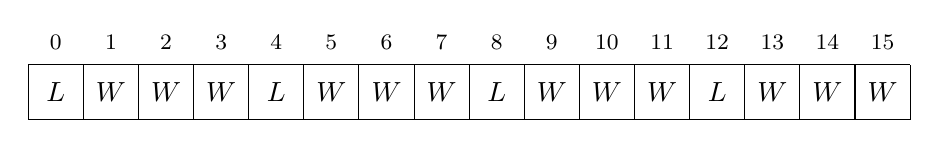
\begin{tikzpicture}[scale=0.7]
\draw (0,0) grid (16,1);

\node at (0.5,0.5) {$L$};
\node at (1.5,0.5) {$W$};
\node at (2.5,0.5) {$W$};
\node at (3.5,0.5) {$W$};
\node at (4.5,0.5) {$L$};
\node at (5.5,0.5) {$W$};
\node at (6.5,0.5) {$W$};
\node at (7.5,0.5) {$W$};
\node at (8.5,0.5) {$L$};
\node at (9.5,0.5) {$W$};
\node at (10.5,0.5) {$W$};
\node at (11.5,0.5) {$W$};
\node at (12.5,0.5) {$L$};
\node at (13.5,0.5) {$W$};
\node at (14.5,0.5) {$W$};
\node at (15.5,0.5) {$W$};

\footnotesize
\node at (0.5,1.4) {$0$};
\node at (1.5,1.4) {$1$};
\node at (2.5,1.4) {$2$};
\node at (3.5,1.4) {$3$};
\node at (4.5,1.4) {$4$};
\node at (5.5,1.4) {$5$};
\node at (6.5,1.4) {$6$};
\node at (7.5,1.4) {$7$};
\node at (8.5,1.4) {$8$};
\node at (9.5,1.4) {$9$};
\node at (10.5,1.4) {$10$};
\node at (11.5,1.4) {$11$};
\node at (12.5,1.4) {$12$};
\node at (13.5,1.4) {$13$};
\node at (14.5,1.4) {$14$};
\node at (15.5,1.4) {$15$};
\end{tikzpicture}
\end{center}

这个游戏很容易分析：
如果 $k$ 能被 4 整除，则状态 $k$ 是必败态，
否则是必胜态。
玩游戏的最优策略是
始终选择一个移动，使得
移动后堆中的火柴数
能被 4 整除。
最终，没有火柴剩下，
对手就输了。

当然，这个策略要求轮到我们时
火柴数\emph{不能}被 4 整除。
如果能被 4 整除，我们无能为力，
如果对手采取最优策略，
对手将赢得游戏。

\subsubsection{状态图}

现在让我们考虑另一个火柴游戏，
在每个状态 $k$ 中，允许移除
任意数量 $x$ 的火柴，
其中 $x$ 小于 $k$ 且整除 $k$。
例如，在状态 8 中我们可以移除
1、2 或 4 根火柴，但在状态 7 中
唯一允许的移动是移除 1 根火柴。

下图展示了游戏的
状态 $1 \ldots 9$ 作为\key{状态图}的形式，
其中节点是状态，边是它们之间的移动：

\begin{center}
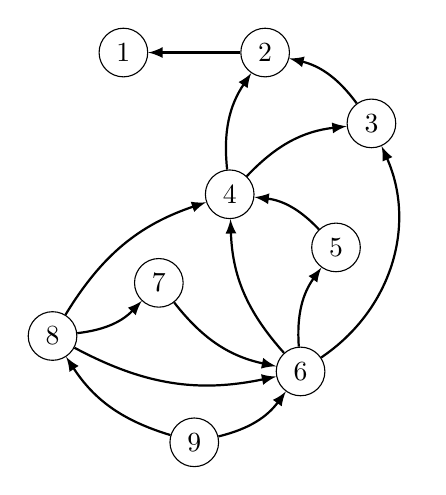
\begin{tikzpicture}[scale=0.9]
\node[draw, circle] (1) at (0,0) {$1$};
\node[draw, circle] (2) at (2,0) {$2$};
\node[draw, circle] (3) at (3.5,-1) {$3$};
\node[draw, circle] (4) at (1.5,-2) {$4$};
\node[draw, circle] (5) at (3,-2.75) {$5$};
\node[draw, circle] (6) at (2.5,-4.5) {$6$};
\node[draw, circle] (7) at (0.5,-3.25) {$7$};
\node[draw, circle] (8) at (-1,-4) {$8$};
\node[draw, circle] (9) at (1,-5.5) {$9$};

\path[draw,thick,->,>=latex] (2) -- (1);
\path[draw,thick,->,>=latex] (3) edge [bend right=20] (2);
\path[draw,thick,->,>=latex] (4) edge [bend left=20] (2);
\path[draw,thick,->,>=latex] (4) edge [bend left=20] (3);
\path[draw,thick,->,>=latex] (5) edge [bend right=20] (4);
\path[draw,thick,->,>=latex] (6) edge [bend left=20] (5);
\path[draw,thick,->,>=latex] (6) edge [bend left=20] (4);
\path[draw,thick,->,>=latex] (6) edge [bend right=40] (3);
\path[draw,thick,->,>=latex] (7) edge [bend right=20] (6);
\path[draw,thick,->,>=latex] (8) edge [bend right=20] (7);
\path[draw,thick,->,>=latex] (8) edge [bend right=20] (6);
\path[draw,thick,->,>=latex] (8) edge [bend left=20] (4);
\path[draw,thick,->,>=latex] (9) edge [bend left=20] (8);
\path[draw,thick,->,>=latex] (9) edge [bend right=20] (6);
\end{tikzpicture}
\end{center}

这个游戏的终态总是状态 1，
这是一个必败态，因为没有
有效的移动。
状态 $1 \ldots 9$ 的分类
如下：

\begin{center}
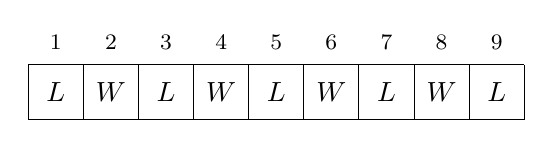
\begin{tikzpicture}[scale=0.7]
\draw (1,0) grid (10,1);

\node at (1.5,0.5) {$L$};
\node at (2.5,0.5) {$W$};
\node at (3.5,0.5) {$L$};
\node at (4.5,0.5) {$W$};
\node at (5.5,0.5) {$L$};
\node at (6.5,0.5) {$W$};
\node at (7.5,0.5) {$L$};
\node at (8.5,0.5) {$W$};
\node at (9.5,0.5) {$L$};

\footnotesize
\node at (1.5,1.4) {$1$};
\node at (2.5,1.4) {$2$};
\node at (3.5,1.4) {$3$};
\node at (4.5,1.4) {$4$};
\node at (5.5,1.4) {$5$};
\node at (6.5,1.4) {$6$};
\node at (7.5,1.4) {$7$};
\node at (8.5,1.4) {$8$};
\node at (9.5,1.4) {$9$};
\end{tikzpicture}
\end{center}

令人惊讶的是，在这个游戏中，
所有偶数状态都是必胜态，
而所有奇数状态都是必败态。

\section{Nim游戏}

\index{Nim游戏}

\key{Nim游戏}是一个简单的游戏，
在博弈论中扮演着重要角色，
因为许多其他游戏都可以使用
相同的策略来玩。
首先，我们关注Nim游戏，
然后将策略推广到其他游戏。

Nim游戏中有 $n$ 个堆，
每个堆包含若干火柴。
玩家交替行动，
每次轮到时，玩家选择
一个仍包含火柴的堆，
并从中移除任意数量的火柴。
移除最后一根火柴的玩家获胜。

Nim游戏的状态形如
$[x_1,x_2,\ldots,x_n]$，
其中 $x_k$ 表示堆 $k$ 中的火柴数。
例如，$[10,12,5]$ 是一个
包含三个堆、分别有10、12和5根火柴的游戏。
状态 $[0,0,\ldots,0]$ 是必败态，
因为无法移除任何火柴，
而这总是最终状态。

\subsubsection{分析}
\index{Nim和}

事实证明，我们可以通过计算
\key{Nim和} $s = x_1 \oplus x_2 \oplus \cdots \oplus x_n$
来轻松分类任何Nim状态，
其中 $\oplus$ 是异或运算\footnote{Nim游戏的最优策略
于1901年由C. L. Bouton发表 \cite{bou01}。}。
Nim和为0的状态是必败态，
所有其他状态是必胜态。
例如，$[10,12,5]$ 的Nim和是
$10 \oplus 12 \oplus 5 = 3$，
所以该状态是必胜态。

但是Nim和与Nim游戏有什么关系呢？
我们可以通过观察Nim状态变化时
Nim和如何变化来解释这一点。

\textit{必败态：}
最终状态 $[0,0,\ldots,0]$ 是必败态，
其Nim和为0，如预期的那样。
在其他必败态中，任何移动都会导致
必胜态，因为当单个值 $x_k$ 发生变化时，
Nim和也会变化，因此移动后的
Nim和不等于0。

\textit{必胜态：}
如果存在任何堆 $k$ 使得 $x_k \oplus s < x_k$，
我们就可以移动到必败态。
在这种情况下，我们可以从堆 $k$ 中移除火柴，
使其包含 $x_k \oplus s$ 根火柴，
这将导致一个必败态。
这样的堆总是存在的，其中 $x_k$
在 $s$ 的最高位的1所对应的位置上
有一个1。

作为例子，考虑状态 $[10,12,5]$。
这个状态是必胜态，
因为其Nim和为3。
因此，必然存在一个移动
可以导致必败态。
接下来我们将找出这样的移动。

该状态的Nim和如下：

\begin{center}
\begin{tabular}{r|r}
10 & \texttt{1010} \\
12 & \texttt{1100} \\
5 & \texttt{0101} \\
\hline
3 & \texttt{0011} \\
\end{tabular}
\end{center}

在这种情况下，含有10根火柴的堆
是唯一一个在Nim和的最高位
1所对应位置上有一个1的堆：

\begin{center}
\begin{tabular}{r|r}
10 & \texttt{10\underline{1}0} \\
12 & \texttt{1100} \\
5 & \texttt{0101} \\
\hline
3 & \texttt{00\underline{1}1} \\
\end{tabular}
\end{center}

堆的新大小必须是
$10 \oplus 3 = 9$，
所以我们只需移除一根火柴。
此后，状态将变为 $[9,12,5]$，
这是一个必败态：

\begin{center}
\begin{tabular}{r|r}
9 & \texttt{1001} \\
12 & \texttt{1100} \\
5 & \texttt{0101} \\
\hline
0 & \texttt{0000} \\
\end{tabular}
\end{center}

\subsubsection{逆向游戏}

\index{逆向游戏}

在\key{逆向游戏}中，游戏的目标
是相反的，
即移除最后一根火柴的玩家
输掉游戏。
事实证明，逆向Nim游戏几乎
可以像标准Nim游戏一样进行最优策略。

思路是先像标准游戏一样进行逆向游戏，
但在游戏结束时改变策略。
新策略将在下一步移动后
每个堆最多包含一根火柴的
情况下引入。

在标准游戏中，我们应该选择一个移动，
使得移动后有偶数个含一根火柴的堆。
然而，在逆向游戏中，我们选择移动使得
有奇数个含一根火柴的堆。

这个策略有效是因为策略发生改变的
状态总是会在游戏中出现，
而这个状态是必胜态，因为它恰好
包含一个超过一根火柴的堆，
所以Nim和不等于0。

\section{Sprague–Grundy定理}

\index{Sprague–Grundy定理}

\key{Sprague–Grundy定理}\footnote{该定理由R. Sprague \cite{spr35}和P. M. Grundy \cite{gru39}独立发现。}将Nim中使用的策略推广到所有满足以下条件的游戏：

\begin{itemize}[noitemsep]
\item 有两名交替行动的玩家。
\item 游戏由状态组成，状态中可能的移动
不取决于轮到谁。
\item 当玩家无法移动时游戏结束。
\item 游戏迟早必定会结束。
\item 玩家对状态和允许的移动有完全信息，
且游戏中没有随机性。
\end{itemize}
思路是为每个游戏状态计算一个Grundy数，
对应于Nim堆中的火柴数。
当我们知道所有状态的Grundy数后，
就可以像Nim游戏一样进行游戏。

\subsubsection{Grundy数}

\index{Grundy数}
\index{mex函数}

游戏状态的\key{Grundy数}是
\[\textrm{mex}(\{g_1,g_2,\ldots,g_n\}),\]
其中 $g_1,g_2,\ldots,g_n$ 是我们可以移动到的
状态的Grundy数，
而mex函数给出不在集合中的
最小非负数。
例如，$\textrm{mex}(\{0,1,3\})=2$。
如果一个状态没有可能的移动，
其Grundy数为0，因为
$\textrm{mex}(\emptyset)=0$。

例如，在状态图
\begin{center}
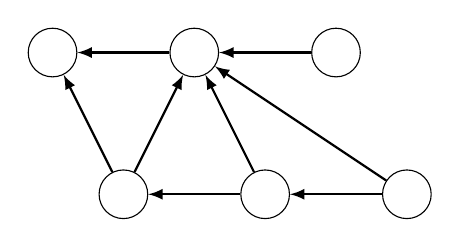
\begin{tikzpicture}[scale=0.9]
\node[draw, circle] (1) at (0,0) {\phantom{0}};
\node[draw, circle] (2) at (2,0) {\phantom{0}};
\node[draw, circle] (3) at (4,0) {\phantom{0}};
\node[draw, circle] (4) at (1,-2) {\phantom{0}};
\node[draw, circle] (5) at (3,-2) {\phantom{0}};
\node[draw, circle] (6) at (5,-2) {\phantom{0}};

\path[draw,thick,->,>=latex] (2) -- (1);
\path[draw,thick,->,>=latex] (3) -- (2);
\path[draw,thick,->,>=latex] (5) -- (4);
\path[draw,thick,->,>=latex] (6) -- (5);
\path[draw,thick,->,>=latex] (4) -- (1);
\path[draw,thick,->,>=latex] (4) -- (2);
\path[draw,thick,->,>=latex] (5) -- (2);
\path[draw,thick,->,>=latex] (6) -- (2);
\end{tikzpicture}
\end{center}
中，Grundy数如下：
\begin{center}
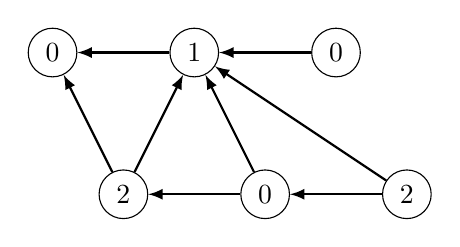
\begin{tikzpicture}[scale=0.9]
\node[draw, circle] (1) at (0,0) {0};
\node[draw, circle] (2) at (2,0) {1};
\node[draw, circle] (3) at (4,0) {0};
\node[draw, circle] (4) at (1,-2) {2};
\node[draw, circle] (5) at (3,-2) {0};
\node[draw, circle] (6) at (5,-2) {2};

\path[draw,thick,->,>=latex] (2) -- (1);
\path[draw,thick,->,>=latex] (3) -- (2);
\path[draw,thick,->,>=latex] (5) -- (4);
\path[draw,thick,->,>=latex] (6) -- (5);
\path[draw,thick,->,>=latex] (4) -- (1);
\path[draw,thick,->,>=latex] (4) -- (2);
\path[draw,thick,->,>=latex] (5) -- (2);
\path[draw,thick,->,>=latex] (6) -- (2);
\end{tikzpicture}
\end{center}
必败态的Grundy数为0，
必胜态的Grundy数为
正数。

状态的Grundy数对应于
Nim堆中的火柴数。
如果Grundy数为0，我们只能移动到
Grundy数为正的状态，
而如果Grundy数为 $x>0$，我们可以移动到
Grundy数包含所有
$0,1,\ldots,x-1$ 的状态。

作为例子，考虑一个玩家
在迷宫中移动棋子的游戏。
迷宫中的每个格子要么是地板要么是墙。
每次轮到时，玩家必须
将棋子向左或向上移动若干步。
做出最后一次移动的玩家获胜。

下图显示了游戏的一个可能的初始状态，
其中 @ 表示棋子，* 表示它可以移动到的格子。

\begin{center}
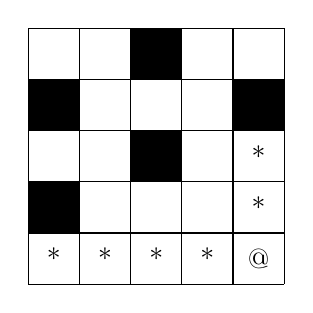
\begin{tikzpicture}[scale=.65]
  \begin{scope}
    \fill [color=black] (0, 1) rectangle (1, 2);
    \fill [color=black] (0, 3) rectangle (1, 4);
    \fill [color=black] (2, 2) rectangle (3, 3);
    \fill [color=black] (2, 4) rectangle (3, 5);
    \fill [color=black] (4, 3) rectangle (5, 4);

    \draw (0, 0) grid (5, 5);
    
    \node at (4.5,0.5) {@};
    \node at (3.5,0.5) {*};
    \node at (2.5,0.5) {*};
    \node at (1.5,0.5) {*};
    \node at (0.5,0.5) {*};
    \node at (4.5,1.5) {*};
    \node at (4.5,2.5) {*};
    
  \end{scope}
\end{tikzpicture}
\end{center}

游戏的状态是迷宫中
所有的地板格子。
在上面的迷宫中，Grundy数
如下：

\begin{center}
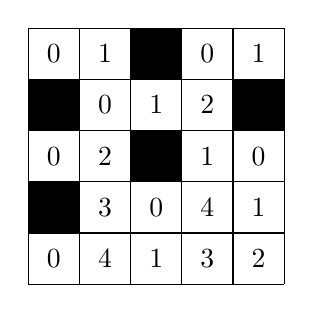
\begin{tikzpicture}[scale=.65]
  \begin{scope}
    \fill [color=black] (0, 1) rectangle (1, 2);
    \fill [color=black] (0, 3) rectangle (1, 4);
    \fill [color=black] (2, 2) rectangle (3, 3);
    \fill [color=black] (2, 4) rectangle (3, 5);
    \fill [color=black] (4, 3) rectangle (5, 4);

    \draw (0, 0) grid (5, 5);
    
    \node at (0.5,4.5) {0};
    \node at (1.5,4.5) {1};
    \node at (2.5,4.5) {};
    \node at (3.5,4.5) {0};
    \node at (4.5,4.5) {1};

    \node at (0.5,3.5) {};
    \node at (1.5,3.5) {0};
    \node at (2.5,3.5) {1};
    \node at (3.5,3.5) {2};
    \node at (4.5,3.5) {};

    \node at (0.5,2.5) {0};
    \node at (1.5,2.5) {2};
    \node at (2.5,2.5) {};
    \node at (3.5,2.5) {1};
    \node at (4.5,2.5) {0};

    \node at (0.5,1.5) {};
    \node at (1.5,1.5) {3};
    \node at (2.5,1.5) {0};
    \node at (3.5,1.5) {4};
    \node at (4.5,1.5) {1};

    \node at (0.5,0.5) {0};
    \node at (1.5,0.5) {4};
    \node at (2.5,0.5) {1};
    \node at (3.5,0.5) {3};
    \node at (4.5,0.5) {2};
  \end{scope}
\end{tikzpicture}
\end{center}

因此，迷宫游戏的每个状态
对应于Nim游戏中的一个堆。
例如，右下角格子的Grundy数为2，
所以它是必胜态。
我们可以通过向左移动四步或
向上移动两步来到达必败态并
赢得游戏。

注意，与原始Nim游戏不同，
有可能移动到一个Grundy数
大于当前状态Grundy数的状态。
然而，对手总是可以选择一个
抵消此移动的移动，因此不可能
从必败态中逃脱。

\subsubsection{子游戏}

接下来我们假设我们的游戏由
子游戏组成，每次轮到时，玩家
先选择一个子游戏，然后在该子游戏中进行一次移动。
当任何子游戏中都无法进行任何移动时，游戏结束。

在这种情况下，游戏的Grundy数
是子游戏Grundy数的Nim和。
通过计算所有子游戏的Grundy数及其Nim和，
可以像Nim游戏一样进行游戏。

作为例子，考虑一个由
三个迷宫组成的游戏。
在这个游戏中，每次轮到时，玩家选择
其中一个迷宫，然后在迷宫中移动棋子。
假设游戏的初始状态如下：

\begin{center}
\begin{tabular}{ccc}
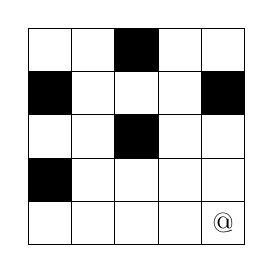
\begin{tikzpicture}[scale=.55]
  \begin{scope}
    \fill [color=black] (0, 1) rectangle (1, 2);
    \fill [color=black] (0, 3) rectangle (1, 4);
    \fill [color=black] (2, 2) rectangle (3, 3);
    \fill [color=black] (2, 4) rectangle (3, 5);
    \fill [color=black] (4, 3) rectangle (5, 4);

    \draw (0, 0) grid (5, 5);

    \node at (4.5,0.5) {@};

    \end{scope}
\end{tikzpicture}
&
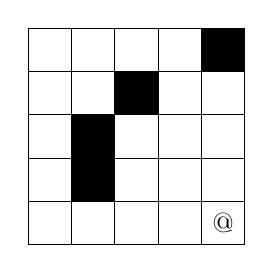
\begin{tikzpicture}[scale=.55]
  \begin{scope}
    \fill [color=black] (1, 1) rectangle (2, 3);
    \fill [color=black] (2, 3) rectangle (3, 4);
    \fill [color=black] (4, 4) rectangle (5, 5);

    \draw (0, 0) grid (5, 5);
    
    \node at (4.5,0.5) {@};

  \end{scope}
\end{tikzpicture}
&
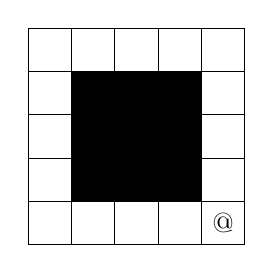
\begin{tikzpicture}[scale=.55]
  \begin{scope}
    \fill [color=black] (1, 1) rectangle (4, 4);

    \draw (0, 0) grid (5, 5);
    
    \node at (4.5,0.5) {@};
  \end{scope}
\end{tikzpicture}
\end{tabular}
\end{center}

迷宫的Grundy数如下：

\begin{center}
\begin{tabular}{ccc}
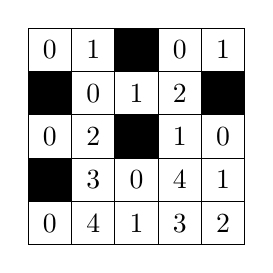
\begin{tikzpicture}[scale=.55]
  \begin{scope}
    \fill [color=black] (0, 1) rectangle (1, 2);
    \fill [color=black] (0, 3) rectangle (1, 4);
    \fill [color=black] (2, 2) rectangle (3, 3);
    \fill [color=black] (2, 4) rectangle (3, 5);
    \fill [color=black] (4, 3) rectangle (5, 4);

    \draw (0, 0) grid (5, 5);

    \node at (0.5,4.5) {0};
    \node at (1.5,4.5) {1};
    \node at (2.5,4.5) {};
    \node at (3.5,4.5) {0};
    \node at (4.5,4.5) {1};

    \node at (0.5,3.5) {};
    \node at (1.5,3.5) {0};
    \node at (2.5,3.5) {1};
    \node at (3.5,3.5) {2};
    \node at (4.5,3.5) {};

    \node at (0.5,2.5) {0};
    \node at (1.5,2.5) {2};
    \node at (2.5,2.5) {};
    \node at (3.5,2.5) {1};
    \node at (4.5,2.5) {0};

    \node at (0.5,1.5) {};
    \node at (1.5,1.5) {3};
    \node at (2.5,1.5) {0};
    \node at (3.5,1.5) {4};
    \node at (4.5,1.5) {1};

    \node at (0.5,0.5) {0};
    \node at (1.5,0.5) {4};
    \node at (2.5,0.5) {1};
    \node at (3.5,0.5) {3};
    \node at (4.5,0.5) {2};
    \end{scope}
\end{tikzpicture}
&
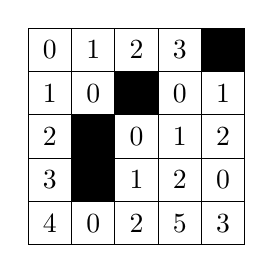
\begin{tikzpicture}[scale=.55]
  \begin{scope}
    \fill [color=black] (1, 1) rectangle (2, 3);
    \fill [color=black] (2, 3) rectangle (3, 4);
    \fill [color=black] (4, 4) rectangle (5, 5);

    \draw (0, 0) grid (5, 5);

    \node at (0.5,4.5) {0};
    \node at (1.5,4.5) {1};
    \node at (2.5,4.5) {2};
    \node at (3.5,4.5) {3};
    \node at (4.5,4.5) {};

    \node at (0.5,3.5) {1};
    \node at (1.5,3.5) {0};
    \node at (2.5,3.5) {};
    \node at (3.5,3.5) {0};
    \node at (4.5,3.5) {1};

    \node at (0.5,2.5) {2};
    \node at (1.5,2.5) {};
    \node at (2.5,2.5) {0};
    \node at (3.5,2.5) {1};
    \node at (4.5,2.5) {2};

    \node at (0.5,1.5) {3};
    \node at (1.5,1.5) {};
    \node at (2.5,1.5) {1};
    \node at (3.5,1.5) {2};
    \node at (4.5,1.5) {0};

    \node at (0.5,0.5) {4};
    \node at (1.5,0.5) {0};
    \node at (2.5,0.5) {2};
    \node at (3.5,0.5) {5};
    \node at (4.5,0.5) {3};
  \end{scope}
\end{tikzpicture}
&
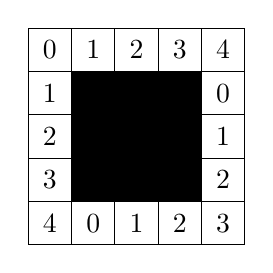
\begin{tikzpicture}[scale=.55]
  \begin{scope}
    \fill [color=black] (1, 1) rectangle (4, 4);

    \draw (0, 0) grid (5, 5);

    \node at (0.5,4.5) {0};
    \node at (1.5,4.5) {1};
    \node at (2.5,4.5) {2};
    \node at (3.5,4.5) {3};
    \node at (4.5,4.5) {4};

    \node at (0.5,3.5) {1};
    \node at (1.5,3.5) {};
    \node at (2.5,3.5) {};
    \node at (3.5,3.5) {};
    \node at (4.5,3.5) {0};

    \node at (0.5,2.5) {2};
    \node at (1.5,2.5) {};
    \node at (2.5,2.5) {};
    \node at (3.5,2.5) {};
    \node at (4.5,2.5) {1};

    \node at (0.5,1.5) {3};
    \node at (1.5,1.5) {};
    \node at (2.5,1.5) {};
    \node at (3.5,1.5) {};
    \node at (4.5,1.5) {2};

    \node at (0.5,0.5) {4};
    \node at (1.5,0.5) {0};
    \node at (2.5,0.5) {1};
    \node at (3.5,0.5) {2};
    \node at (4.5,0.5) {3};
  \end{scope}
\end{tikzpicture}
\end{tabular}
\end{center}

在初始状态中，Grundy数的Nim和
为 $2 \oplus 3 \oplus 3 = 2$，
所以先手玩家可以赢得游戏。
一个最优移动是在第一个迷宫中
向上移动两步，这产生Nim和
$0 \oplus 3 \oplus 3 = 0$。

\subsubsection{Grundy游戏}

有时游戏中的一次移动会将游戏
划分为相互独立的子游戏。
在这种情况下，游戏的Grundy数是

\[\textrm{mex}(\{g_1, g_2, \ldots, g_n \}),\]
其中 $n$ 是可能的移动数，
\[g_k = a_{k,1} \oplus a_{k,2} \oplus \ldots \oplus a_{k,m},\]
其中移动 $k$ 生成Grundy数为
$a_{k,1},a_{k,2},\ldots,a_{k,m}$ 的子游戏。

\index{Grundy游戏}

这类游戏的一个例子是\key{Grundy游戏}。
最初，有一个包含 $n$ 根火柴的堆。
每次轮到时，玩家选择一个堆并将其
划分为两个非空堆，使得两个堆
的大小不同。
做出最后一次移动的玩家获胜。

设 $f(n)$ 为包含 $n$ 根火柴的堆的Grundy数。
Grundy数可以通过遍历将堆划分为
两个堆的所有方式来计算。
例如，当 $n=8$ 时，可能的划分为
$1+7$、$2+6$ 和 $3+5$，所以
\[f(8)=\textrm{mex}(\{f(1) \oplus f(7), f(2) \oplus f(6), f(3) \oplus f(5)\}).\]

在这个游戏中，$f(n)$ 的值基于
$f(1),\ldots,f(n-1)$ 的值。
基本情况是 $f(1)=f(2)=0$，
因为无法划分包含1根和2根火柴的堆。
前几个Grundy数为：
\[
\begin{array}{lcl}
f(1) & = & 0 \\
f(2) & = & 0 \\
f(3) & = & 1 \\
f(4) & = & 0 \\
f(5) & = & 2 \\
f(6) & = & 1 \\
f(7) & = & 0 \\
f(8) & = & 2 \\
\end{array}
\]
$n=8$ 的Grundy数为2，
所以有可能赢得游戏。
获胜的移动是创建堆
$1+7$，因为 $f(1) \oplus f(7) = 0$。

